%%%%%%%%%%%%%%%%%%%%%%%%%%%%%%%%%%%%%%%%%%%%%%%%%%%%%%%%%%%%%%%%%%%%%%%%%%%%%%%%%
%
% Purpose:  Validation part of V&V for the SolarBeta model
%
%
%
%%%%%%%%%%%%%%%%%%%%%%%%%%%%%%%%%%%%%%%%%%%%%%%%%%%%%%%%%%%%%%%%%%%%%%%%%%%%%%%%

\section{Validation}

\test{Comparison with External Data}
\label{test:solarbetacompare}
\begin{description}
\item{Purpose:} \\
The purpose of this test is to compare solar beta angles
calculated by this model with externally-provided values.

\item{Requirements:} \ \newline
The succesful outcome of this test, together with the validation Test~\ref{test:solarbetalongterm} satisfy requirement~\ref{reqt:SolarBeta}.

\item{Procedure:}\ \newline
Several tests are carried out, including:
\begin{enumerate}
\item{RUN\_comp\_ISS} \ \newline
This run compares against the Solar Beta for ISS, using a simple ephemeris model.
The reference data from The Flight Operation Directorate at NASA JSC 
provides a solar beta value for a given ISS state (inertial position/velocity)
at a given date. The underlying program uses a simple ephemeris model,
resulting in solar beta angles accurate to within 1 degree.
The vehicle state and time as portrayed in
Figure~\ref{fig:STS_114_ISS} were used to initialize the test simulation
and to validate the results.

\begin{figure}
\centering
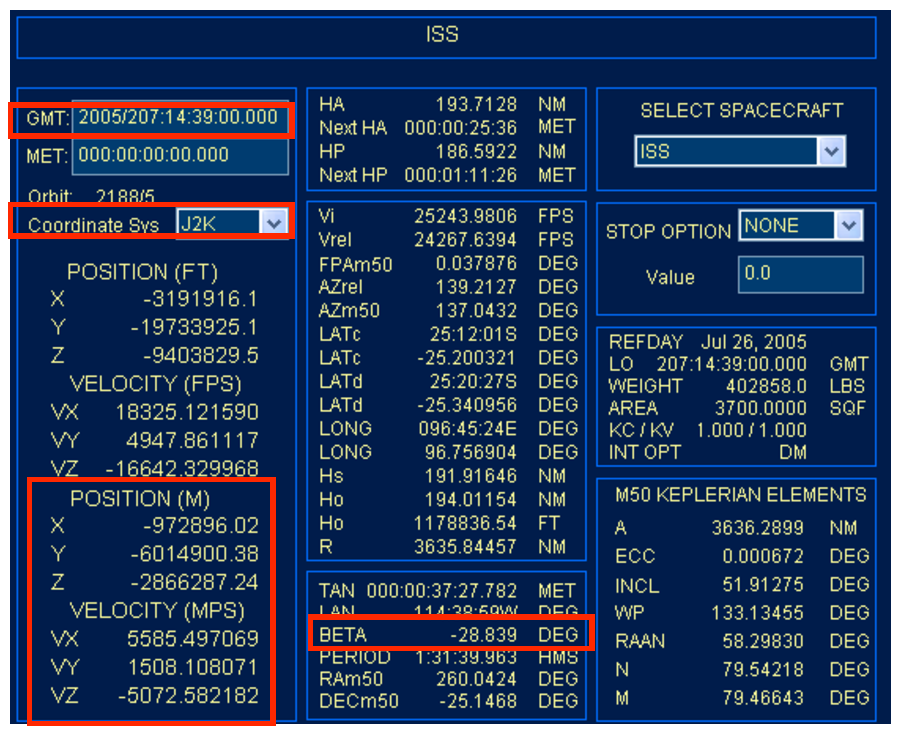
\includegraphics{figures/SOLAR_BETA_fig5}
\caption{Mission Operations ISS State and Solar Beta}
\label{fig:STS_114_ISS}
\end{figure}

\item{RUN\_comp\_STS121a and RUN\_comp\_STS121b] STS-121} \ \newline
These runs compare against the Solar Beta for ISS, generated using the DE405 ephemeris
The Mission Operations Directorate uses the DE405 ephemeris
to compute solar beta angles in flight-certified applications.
Mission STS-121 data, provided by William H. Tracy/NASA/JSC/DM32,
provided solar beta values for a pair of given STS-121 states.

The vehicle state and time as portrayed in
figures~\ref{fig:STS_121a} and~\ref{fig:STS_121b} were used to initialize
the test simulation and to validate the results.
\end{enumerate}

\item{Predictions:}
\begin{enumerate}
\item{RUN\_comp\_ISS} \ \newline
The Solar Beta angles generated by the
simple ephemeris model are accurate to within one degree compared to
angles computed with the aid of the highly accurate DE405 ephemeris model.

Therefore, the solar beta angle computed using the \SolarBetaDesc\ should differ with
the externally-provided value by no more than one degree
for this test case.

\item{RUN\_comp\_STS121a and RUN\_comp\_STS121b}\ \newline
Solar beta angles generated externally using the DE405 ephemeris model
should agree with angles computed by the \SolarBetaDesc\ to a very high degree.
The validation data for these tests provide initial conditions in the M50 reference frame, whereas \JEODid\ uses the J2000 frame.  A conversion of the specification state from M50 to J2000 serves as the initialization data for these tests.  This incorporates a potential source of error.
Other sources of error are in the state vector and the epoch time.
The externally-provided data give solar beta angles with three
decimal places of precision (that is, $1/1000^{th}$ degree).  The initial state and Solar Beta angle for these two tests are shown in Figures~\ref{fig:STS_121a} and~\ref{fig:STS_121b}.

Even accounting for the potential errors introduced by the precision in the specification of the epoch time, and of the M50 state, and further, its conversion to J2000 conversion, the solar beta angle computed using the \SolarBetaDesc\ should differ with the externally-provided value by no more than $0.001^\circ$ for these test cases.
\end{enumerate}

\item{Results:}
\begin{enumerate}
\item{RUN\_comp\_ISS}\\
 The solar beta angle calculated by the simulation at
initialization time was $-28.41^\circ$, which, to within $1^\circ$,
agrees with the externally- supplied value of $-28.839^\circ$.

\item{RUN\_comp\_STS121a and RUN\_comp\_STS121b} \\
The solar beta angles calculated by the simulation at initialization time are
$5.29269^\circ$ (RUN\_comp\_STS121a) and $3.85718^\circ$ (RUN\_comp\_STS121b),
which, to $0.001^\circ$, compare exactly the externally-supplied values
of $5.293^\circ$ and $3.857^\circ$
\end{enumerate}
All test cases pass their respective test criterion.
\end{description}


\begin{figure}
\centering
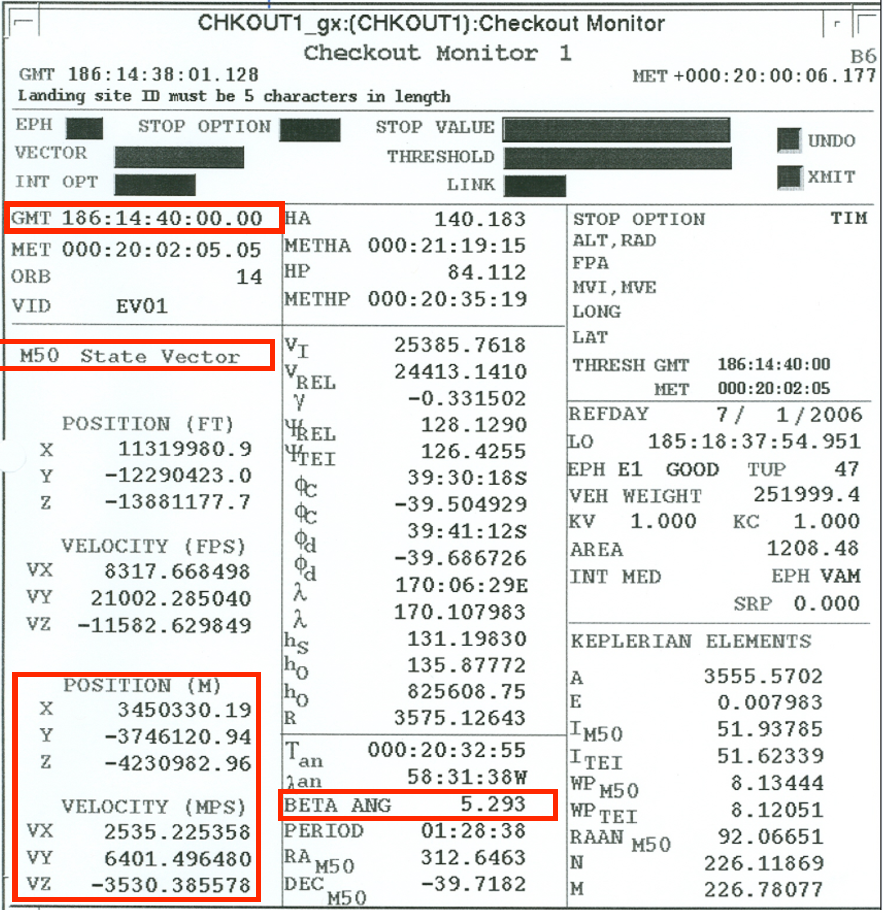
\includegraphics{figures/SOLAR_BETA_fig6}
\caption{Mission Operations STS-121 Checkout Monitor Data}
\label{fig:STS_121a}
\end{figure}


\begin{figure}
\centering
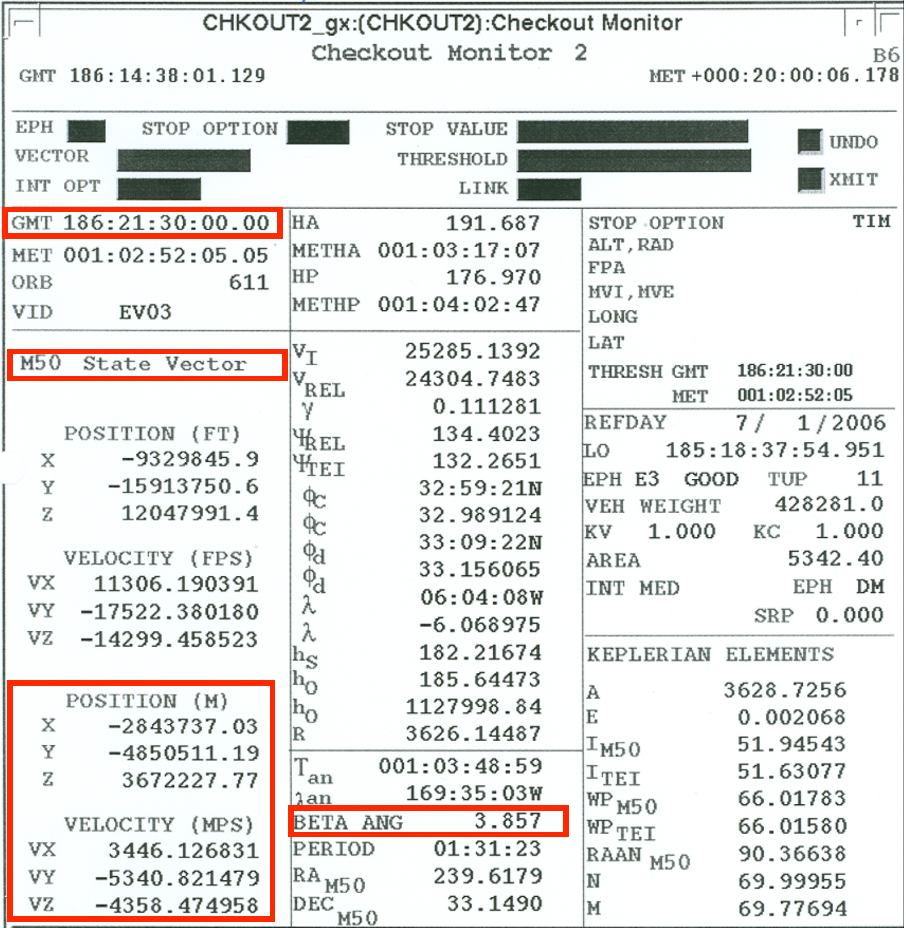
\includegraphics{figures/SOLAR_BETA_fig7}
\caption{Mission Operations STS-121 Checkout Monitor Data}
\label{fig:STS_121b}
\end{figure}

\clearpage
